\section{Methods}
\label{sec:Methods}
In our work, we describe about two user studies. First, we collected data using the eye-tracker device which is similar to Alam et al.~\cite{alamdata}. Second, we conducted a user study where users look at the data of the first users'. At the first user study, we constructed PivotPaths diagram~\cite{dork2012pivotpaths} using IMDB ( Internet Movie DataBase) data. Similar to Alam et al.~\cite{alamdata}, the users were able to search movies, actors, and directors. Whenever, a user selected a actors or director, we generate a PivotPaths diagram using top rated movies of that person along with other actors, directors, genres. However if a movie was selected, the PivotPaths diagram got generated with a list of movies having the most common elements of that movie. Figure~\ref{fig:pivotpaths} shows a PivotPaths diagram where the movie ``Raiders of the lost ark'' is selected. 
\begin{figure}[htb]
  \centering
  \includegraphics[width=\linewidth]{images/pivotpaths.eps}
  \caption{PivotPaths visualization of IMDB data. Movies are displayed in the center of the screen, actors at the top, and directors and genres share the bottom space. Actors, directors, and genres associated to movies are connected through curves. Users can highlight objects and their connected neighbors by hovering over them.}
	\label{fig:pivotpaths}
\end{figure}

We used the instrumentation of Alam et al. The eye-tracker data consisted with a list of data objects with the time, id, type and a score calculated using the instrumentation. 

At the second user study, we developed a time-line visualization. As in the eye-tracker data we have a list of data objects with scores, for particular time $t$ we calculated the top 10 data objects which the user was likely seeing in $t-90$ seconds. For that implementation, we simply aggregated the data object list and sorted them based on their scores and provided priority to the data objects with more later time. After calculating the data objects we generate labels with height according to their weighted score over $t-90$ seconds. After generating the labels we generate the heatmap similar to Alam et al. to get a sense when a first users was looking at a data object. Figure~\ref{fig:heatmap} shows an instance of the timeline visualization.
\begin{figure}[htb]
  \centering
  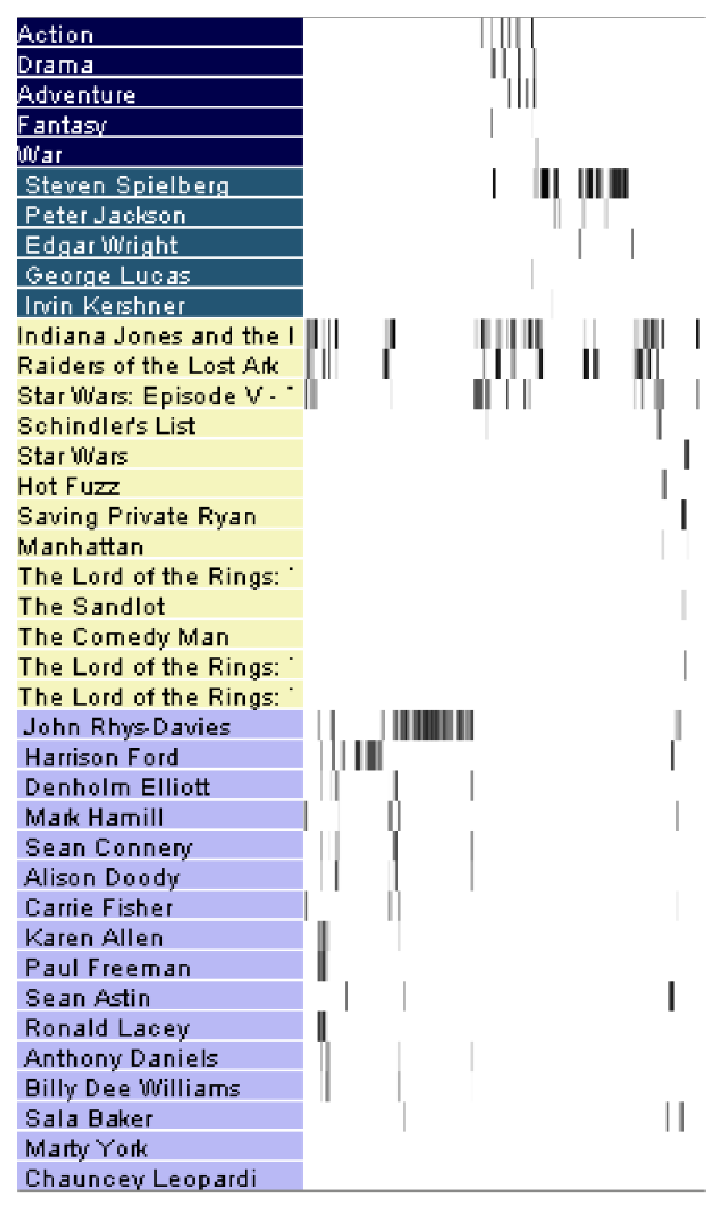
\includegraphics[width=\linewidth]{images/heatmap.eps}
  \caption{A time-line visualization for the second user study.}
	\label{fig:heatmap}
\end{figure}
